\chapter{Introduction}

Laser frequency stabilisation is an essential tool for atomic physics experiments, without it experiments involving \glspl{bec}, atomic clocks and many more would not be possible~\cite{anderson_observation_1995,ye_quantum_2008}.
There are a plethora of techniques available for laser frequency stabilisation each with numerous advantages and disadvantages.

\Gls{ps} is one such technique that will be discussed in detail~\cite{demtroder_laser_2003}.
\Gls{ps} was first described by Wieman and H\"anch in 1976 as, ``...a sensitive new method of Doppler-free spectroscopy, monitoring the nonlinear interaction of two monochromatic laser beams in an absorbing gas via changes in light polarisation."~\cite{wieman_doppler-free_1976}
This chapter provides an overview of laser frequency stabilisation, a detailed discussion of the physics of \gls{ps} followed by details on the implementation and measurement of high bandwidth frequency stabilisation using \gls{ps}.

{\color{red} Mention Rb context and other common elements used in laser cooling.}

\section{Laser Frequency Stabilisation}

Laser frequency stabilisation describes a number of techniques that are used to reduce the temporal frequency spread of a laser's frequency.
This can range from weak frequency stabilisation keeping the centre frequency of a laser at a particular point to convoluted frequency narrowing techniques that attempt to reduce laser linewidth to sub-hertz levels.
Typically these techniques use some reference to measure frequency deviation from a given frequency and provide negative feedback to the laser, using a servo system, to keep it at the target frequency.

The efficacy of stabilisation techniques can be described by width of the frequency distribution of the laser, called the linewidth.
Width is usually refers to either the \gls{fwhm} or \gls{rms} width about the central frequency.
Linewidth can describe short or long timescale measurements.
Short measurements, usually less than a second measurement, are used to describe the linewidth of laser whereas long timescale measurement, hours or days in duration, are used to describe the drift of the laser central frequency over time.

There are a number of traits that are desirable in a laser frequency stabilization scheme including the ability to stabilize to an absolute atomic reference, absence of frequency or amplitude modulation, high bandwidth to achieve low spectral linewidth, large capture range, low complexity and low cost.

There are a large number of available techniques and variations on techniques for stabilization each with different advantages and drawbacks.
A few of these techniques are listed below:
\begin{itemize}
\item \gls{sa}~\cite{haroche_theory_1972, maguire_theoretical_2006, cuneo_optically_1994, preston_doppler-free_1996, saliba_linewidths_2009},
\item \gls{davll}~\cite{corwin_frequency-stabilized_1998, millett-sikking_davll_2007},
\item \gls{mts}~\cite{shirley_modulation_1982, mccarron_modulation_2008, xiang-hui_ultra-stable_2009},
\item Sagnac interferometry~\cite{robins_Interferometric_2002, jundt_non-linear_2003},
\item \acrfull{ps}~\cite{wieman_doppler-free_1976, lancaster_polarisation_1999, yoshikawa_frequency_2003, harris_polarization_2006, pearman_polarization_2002, tiwari_laser_2006, do_polarization_2008, torii_laser-phase_2012}
\item \gls{pdh}~\cite{drever_laser_1983} and
\item H\"ansch Couillaud stabilisation~\cite{hansch_laser_1980}.
\end{itemize}
Some of these techniques will be discussed later on in this chapter.

\section{Frequency Control and Feedback}

There are a number of ways to control the output frequency of a laser and these methods can be used to supply feedback from the stabilisation technique in order to decrease the linewidth of a laser system.
The focus here will be on the feedback systems of diode lasers, particularly \glspl{ecdl}.

\subsection{Temperature}
The temperature of a laser diode affects the output frequency due to the temperature dependence of the optical path length and gain curves~\cite{wieman_using_1991}.
The two processes affect output frequency at different rates and both show an increase in wavelength with increasing temperature.

The temperature of laser diodes can be controlled through two methods. \Glspl{tec} can be used to directly control the temperature of the device and the injection current into the diode affects the temperature. Good insulation and thermal inertia also contribute to the stability of diode temperature~\cite{saliba_cold_2011}.

\subsection{Injection Current}
Modulation of the injection current into the laser diode is one of most common ways of controlling the output wavelength of a diode laser.
The injection current into the diode affects the temperature of the diode and the density of charge carriers which in turn affects the refractive index of the medium and thus the wavelength of the laser light produced.

The design of the electronics involved in the modulation of the injection current can have a noticeable influence on the performance at high frequencies as noise becomes an issue.
{\color{red} Citations or more discussion.}

\subsection{Grating Angle}
In external cavity diode lasers, for example Littrow configuration \glspl{ecdl} as shown in Fig.~\ref{figure:littrow}, the angle of the external grating can be used to control the output frequency.
The grating angle affects the wavelength of the light that is reflected back into the laser diode and thus the angle can be used to select output wavelength.
The grating angle is commonly controlled using piezoelectric actuators~\cite{hawthorn_littrow_2001}.

\begin{figure}
\includegraphics[width=\linewidth]{part1/Figs/littrow.jpg}
\caption{Littrow configuration for diode lasers.}
\label{figure:littrow}
\end{figure}

{\color{red} Verify these and provide citations.}
To talk about:
\begin{itemize}
\item Typical feedback bandwidths.
\item Fast feedback - complications (isolation from ground, phase lag...).
\end{itemize}


\section{Noise}
Thermal noise can affect the alignment of optics, the efficiency and polarisation of light transmitted through fibres, atomic vapour cell opacity and the intensity and frequency of light emitted from laser diodes, not to mention mode hops.

Noise in the electronic environment can also cause frequency instability. Noise on the power supply to the laser diode affects the intensity and frequency of the light emitted.

In certain applications {\color{red}(such as?? imaging?)} intensity noise can be as much as a drawback as frequency noise and with some frequency discrimination methods intensity noise is interpreted as frequency noise which the servo would then attempt to correct for thus inducing frequency noise.

Feedback to laser systems typically takes the form of modulation of either the current supply to the diode or the voltage to a piezo that controls the angle of the grating in an \gls{ecdl}.
Temperature feedback has also been used to maintain frequency stability {\color{red}[find that paper again]}.
The bandwidth of current feedback tends to range from \unit[0]{Hz} to MHz~\cite{ludlow_compact_2007}{\color{red}[cite my paper here?]}.
Piezo response is significantly slower ranging from \unit[0]{Hz} to \unit[100]{kHz}.

{\color{red}Frequency ranges of noise.}

{\color{red}More detail? More References on noise in general.}

{\color{red}Cite some of Seb's stuff thesis\cite{saliba_cold_2011}, papers\cite{saliba_linewidths_2009, saliba_mode_2009}.}

Bleh.
\Glspl{ecdl} subjected to mechanical vibrations will experience frequency noise as the alignment of the light coupled back into the diode off the grating varies.
Vibrations can also affect the alignment, and thus transmitted power, of laser through optical fibres, optical isolators and through apertures.

\section{Stabilisation Techniques}

This section contains a brief overview of a number of stabilisation techniques.

\subsection{Saturated Absorption Spectroscopy}
\Gls{sa} is a simple and common technique for laser frequency stabilisation~\cite{demtroder_laser_2003}.
The technique is occasionally used in undergraduate experiments and is used with a number of atomic species.
\Gls{sa} is often used in experiments where narrow linewidths are not required due to the ease and setup and low cost.

\Gls{sa} can be a DC or AC stabilization technique.
The DC technique is more susceptible to drift and there is an frequency offset from the atomic transition whereas the AC technique requires the added complexity of modulation of the laser frequency and the linewidth is limited by modulation frequency.
Linewidths under 150\,kHz are easily attainable with AC saturated absorption spectroscopy.

{\color{red}Explain DC/AC.}

{\color{red}Sat abs spectrum}
 
\begin{figure}
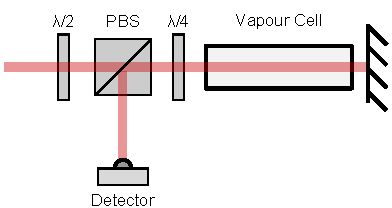
\includegraphics[width=\linewidth]{part1/Figs/SatAbs.pdf}
\caption{An example of a saturated absorption spectroscopy setup.}
\label{figure:satabs}
\end{figure}

\begin{figure}
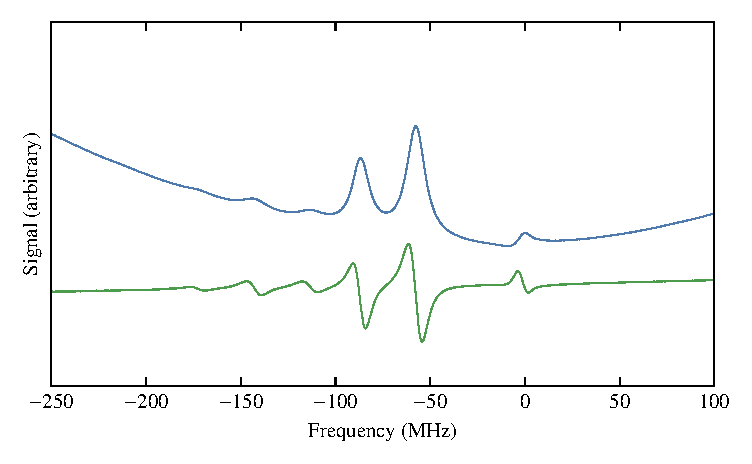
\includegraphics[width=\linewidth]{part1/Figs/SatAbsSpectrum.pdf}
\caption{An example of a saturated absorption spectroscopy spectrum for the rubidium-85 D2 transition.}
\label{figure:satabsspectrum}
\end{figure}

\subsection{Polarisation Spectroscopy}

Summary of PS.

Pol Spec developments

It has been shown previously that \gls*{ps} can be used to reduce the linewidth of a distributed feedback diode from \unit[2]{MHz} to \unit[20]{kHz}~\cite{torii_laser-phase_2012} and of \glspl*{ecdl} to \unit[65]{kHz}
~\cite{yoshikawa_frequency_2003}.

Balanced polarimeter.\cite{pearman_polarization_2002,yoshikawa_frequency_2003}

Bi-polarisation spectroscopy.\cite{tiwari_laser_2006}


\subsection{Pound Drever Hall}

The \gls{pdh} technique is the standard for laser frequency linewidth reduction.\cite{drever_laser_1983}
\gls{pdh} uses an optical cavity as a frequency reference and an \gls{eom} to modulate the the light incident to the cavity.

More detail. Some maths. What linewidth can it achieve?\cite{ludlow_compact_2007}

\begin{figure}
\centering
\includegraphics[width=\linewidth]{part1/Figs/pdh.jpg}
\caption{A beautiful \gls{pdh} schematic.}
\end{figure}
\subsubsection{Dichroic Atomic Vapour Laser Lock}
\Gls{davll} works by....

It can achieve linewidths of....

\subsection{Modulation Transfer Spectroscopy}
\Gls{mts}...

It can achieve linewidths of...\cite{negnevitsky_wideband_2013}

\subsection{Other Techniques}

Any others?


